\documentclass[14pt, a4paper]{article}
\usepackage[russian]{babel}
\usepackage{graphicx}
\usepackage{layout}
\usepackage[14pt]{extsizes}
\usepackage{amssymb}
\usepackage{relsize}

\setcounter{tocdepth}{4}
\setcounter{secnumdepth}{4}

\usepackage{xcolor}
\usepackage{hyperref}

\usepackage{listings}

 % Цвета для гиперссылок
\definecolor{linkcolor}{HTML}{000000} % цвет ссылок
\definecolor{urlcolor}{HTML}{000000} %цвет гиперссылок

\hypersetup{pdfstartview=FitH,  linkcolor=linkcolor,urlcolor=urlcolor, colorlinks=true}

\definecolor{codegreen}{rgb}{0,0.6,0}
\definecolor{codegray}{rgb}{0.5,0.5,0.5}
\definecolor{codepurple}{rgb}{0.58,0,0.82}
\definecolor{backcolour}{rgb}{0.97,0.97,0.97}

%таблица
\lstdefinestyle{mystyle}{
    backgroundcolor=\color{backcolour},   
    commentstyle=\color{codegreen},
    keywordstyle=\color{magenta},
    numberstyle=\tiny\color{codegray},
    stringstyle=\color{codepurple},
    basicstyle=\ttfamily\footnotesize,
    breakatwhitespace=false,         
    breaklines=true,                 
    captionpos=b,                    
    keepspaces=true,
    frame=single,                                                    
    showspaces=false,                
    showstringspaces=false,
    showtabs=false,                  
    tabsize=2,
    mathescape=true
}

\lstset{style=mystyle}

%Разметка страницы
\oddsidemargin = 0pt
\marginparwidth = 45pt 
\textwidth = 467pt
\textheight = 716pt
\topmargin = 0pt 
\footskip = 30pt 
\headheight = 0pt 
\headsep = 0pt 

\begin{document}
\begin{titlepage}
    \topmargin=216pt
    \newpage
    \hangindent=0.7cm
    \huge ИУ-10\\
    Системное\\
    Программное\\
    Обеспечение\\
    Администрирование Linux\\
    \textbf{Процессы.\\
    Systemd и его возможности.}

    \vspace{9cm}

    \begin{center}
        \small\textit{Москва, 2022}
    \end{center}
\end{titlepage}

\section*{На этом уроке} 
\addcontentsline{toc}{section}{На этом уроке}

\begin{enumerate}
    \item Узнаем, как происходит процесс загрузки ОС.
    \item Выясним, что такое процесс и как управлять процессами.
    \item Познакомимся с главным процессом в системе - systemd
    \item Разберём простейшие утилиты мониторинга процессов.
\end{enumerate}


\tableofcontents
\newpage

\section*{Процесс} 
\addcontentsline{toc}{section}{Процесс}

Для всего, что происходит на сервере Linux, запускается процесс. Процесс - это совокупность кода,
выполняющегося в памяти компьютера. Есть приложения, которые могут создавать в результате
своей работы не один, а несколько процессов. Когда процесс запущен, он может использовать
несколько потоков (thread). Поток - это задача, запускаемая процессом, которую может обслуживать
выделенное ядро процессора.\\

\noindent Можно выделить три основных типа процессов:
\begin{itemize}
    \item[-] Пользовательские процессы (shell job) - это команды, запускаемые из командной строки. Они
    связаны с оболочкой, которая была текущей на момент запуска процесса.
    \item[-] Демоны - это процессы, предоставляющие сервисы. Обычно они запускаются при загрузке
    системы и часто (но, конечно, не во всех случаях) запускаются с правами root.
    \item[-] Потоки ядра являются частью ядра Linux. Вы не можете управлять ими с помощью обычных
    инструментов, но для мониторинга производительности системы важно за ними следить.
\end{itemize}

\noindent Процесс может находиться в разных состояниях. Вот некоторые из них:
\begin{enumerate}
    \item Процесс работает — состояние когда код процесса выполняется.
    \item Процесс «спит» — состояние, когда процесс ожидает каких-то событий (ввода данных с
    клавиатуры и т. п.).
    \item Процесс остановлен — процесс был остановлен, чаще всего при помощи сигналов.
    \item Процесс «зомби» — процесс уже не существует, его код и данные уже выгружены из
    оперативной памяти компьютера, но запись в таблице процессов сохранилась. \textbf{Примечание!}
    \underbar{\textit{Подобное состояние процессов}} \\
    \underbar{\textit{крайне не желательно.}}
\end{enumerate}

\subsection*{Атрибуты процессов} 
\addcontentsline{toc}{subsection}{Атрибуты процессов}

У каждого процесса есть набор важных атрибутов:
\begin{enumerate}
    \item \href{https://rtfm.co.ua/unix-pid-ppid-i-nohup/}{\textbf{PID и PPID}} — идентификатор процесса (Process Identifier) и идентификатор родительского
    процесса (Parent Process Identifier). Числовое значение, присваиваемое каждому процессу: от
    1 до 65535. Процессы в ОС Linux имеют древовидную структуру. При старте запускается
    процесс systemd с номером 1, который порождает все остальные процессы. Процесс получает
    при запуске свои \textbf{PID} и \textbf{PPID}. PID процесса всегда уникален, но при этом у нескольких
    процессов может быть одинаковый \textbf{PPID}. Операционная система взаимодействует с
    процессами через \textbf{PID}.
    \item \textbf{UID} — владелец процесса, пользователь, от которого запущен процесс.
    \item \textbf{TTY} - терминал, из которого запущен процесс
    \item \textbf{TIME} - общее время процессора, затраченное на выполнение процессора
    \item \textbf{CMD} — команда, запустившая процесс.
\end{enumerate}

Список запущенных процессов и указанных атрибутов позволит увидеть команда \textbf{ps -ef}.
\vspace{0.3cm}

\begin{lstlisting}
root@server:$\sim$# ps -ef | grep -P

UID        PID    PPID C STIME TTY        TIME CMD

root        655        1  0 Jan08 ?       00:00:00 sshd: /usr/sbin/sshd -D
[listener] 0 of 10-100

root      5413    655  0 08:54 ?          00:00:00 sshd: user

\end{lstlisting}

\subsection*{Сигналы} 
\addcontentsline{toc}{subsection}{Сигналы}

Пользовательские процессы, как правило, живут до окончания пользовательской сессии, но бывают
случаи, когда какое-то приложение или запущенный процесс необходимо завершить аварийно (оно
банально зависло). Такие ситуации возникают не только с пользовательскими процессами, но и с
процессами-демонами. Для завершения работы существуют специальные сигналы, которые мы
можем передать процессу, используя команду \textbf{kill}. Полный список сигналов можно получить,
выполнив команду \textbf{kill -l}.\\

\noindent Из \href{https://ru.wikipedia.org/wiki/Сигнал_(Unix)}{28 сигналов} стоит выделить следующие три:
\begin{itemize}
    \item[-] Сигнал \textbf{SIGTERM (15)} используется для запроса остановки процесса.
    \item[-] Сигнал \textbf{SIGKILL (9)} используется для принудительной остановки процесса.
    \item[-] Сигнал \textbf{SIGHUP (1)} используется для приостановки процесса. В результате процесс
    перечитывает свои файлы конфигурации, что делает этот сигнал полезным для внесения
    изменений в файл конфигурации процесса.
\end{itemize}

Команда \textbf{kill} работает с процессом через его \textbf{PID} или \textbf{PPID}. \colorbox{backcolour}{kill -15} 
\colorbox{backcolour}{<PID>} посылает процессу сигнал SIGTERM, который обычно заставляет процесс прекращать свою деятельность и в спокойном
режиме закрывать все открытые файлы.\\

Сигнал SIGTERM работает не всегда, потому что процессы имеют право его игнорировать (условия
игнорирования определяются разработчиками ПО). В этом случае используется \colorbox{backcolour}{kill -9 <PID>},
чтобы послать процессу сигнал \textbf{SIGKILL}. Поскольку сигнал SIGKILL нельзя игнорировать, он
заставляет процесс останавливаться в любой ситуации, даже с риском потери данных. Помимо этого,
передав сигнал на принудительное завершение \textbf{PPID} (ID родительского процесса) \colorbox{backcolour}{kill -9 <PPID>},
мы завершим всё дерево процессов, порождённых этим процессом, что может сильно
дестабилизировать систему.

\vspace{0.3cm}

\begin{lstlisting}
root@server:$\sim$# ps -ef | grep nginx

root          $\mathbf{702}$         1  0 16:05 ?          00:00:00 nginx: master

/usr/sbin/nginx -g daemon on; master_process on;

www-data    703     $\mathbf{702}$ 0 16:05 ?         00:00:00 nginx: worker

root       1408     987 0 17:38 pts/0     00:00:00 grep --color=auto nginx

root@server:$\sim$# kill -9 702

root@server:$\sim$# ps -ef | grep nginx

root       1410     987 0 17:39 pts/0     00:00:00 grep --color=auto nginx

root@server:$\sim$#
$$
\end{lstlisting}
\vspace{0.2cm}

В этом примере мы нашли PID процесса - 702, у которого есть дочерний процесс - 703. Передав \colorbox{backcolour}{kill
-9} 702 , мы убили сразу оба процесса.

\section*{Systemd} 
\addcontentsline{toc}{section}{Systemd}

Systemd - это самый масштабный процесс, который управляет запуском оборудования,
монтированием файловых систем, стартом служб, ограничением потребления ресурсов и многим
другим. По сути это менеджер всего в User Space.\\

Важным в работе systemd является понятие юнита. Юнит или модуль - это абстрактный элемент,
попадающий под управление systemd. Юнитом могут быть службы, точки монтирования, сервисы,
работающие по времени, и многое другое.\\

\noindent Полный перечень юнитов можно получить с помощью команды \colorbox{backcolour}{systemctl -t}
\colorbox{backcolour}{help}.
\vspace{0.3cm}

\begin{lstlisting}
root@server:$\sim$# systemctl -t help
Available unit types:
service
mount
swap
socket
target
device
automoun
t timer
path
slice
scope
$$
\end{lstlisting}
\vspace{0.2cm}

\textbf{Systemctl} — основная команда для управления и мониторинга \textbf{systemd}, позволяет получать
информацию о состоянии системы и запущенных службах, а также управлять службами.\\

Основные параметры \textbf{systemctl}:
\begin{enumerate}
    \item \colorbox{backcolour}{systemctl status} выведет на экран состояние системы.
    \item \colorbox{backcolour}{systemctl} выведет список запущенных юнитов.
    \item \colorbox{backcolour}{systemctl [start|stop|status|restart|reload] service\_name} позволит запустить
    службу (start), остановить (stop), получить информацию о службе (status), перезапустить
    службу (restart), перечитать конфигурационный файл службы (reload).
\end{enumerate}

\begin{lstlisting}
root@server:$\sim$# systemctl status nginx.service
$\bullet$ nginx.service - A high performance web server and a reverse proxy server
    Loaded: loaded (/lib/systemd/system/nginx.service; disabled; vendor 
preset: enabled)
    Active: active (running) since Wed 2021-01-06 21:16:21 UTC; 2 days ago
      Docs: man:nginx(8)
  Main PID: 659 (nginx)
     Tasks: 2 (limit: 2282)
    Memory: 11.6M
    CGroup: /system.slice/nginx.service
                 $\mathlarger{\mathlarger{\vdash}}$659 nginx: master process /usr/sbin/nginx -g daemon on;
master_process on;
             $ {^\mathlarger{\mathlarger{{\mathlarger{\llcorner}}}}} $661 nginx: worker process

Jan 06 21:16:20 server systemd[1]: Starting A high performance web server 
and a reverse proxy server...
Jan 06 21:16:21 server systemd[1]: Started A high performance web server 
and a reverse proxy server.
$$
\end{lstlisting}

\vspace{0.2cm}

\noindent \textbf{Примечание!} \underbar{\textit{Служба \colorbox{backcolour}{nginx.service} является примером юнита systemd}}. Из вывода можно
получить информацию о состоянии процесса, времени работы, используемой памяти,
небольшую часть логов.

\begin{enumerate}
    \item[4.] \colorbox{backcolour}{systemctl [enable|disable] service\_name} позволит добавить (enable) или убрать
    (disable) службу из автозагрузки.
\end{enumerate}

\subsection*{Файлы Модулей/Юнитов} 
\addcontentsline{toc}{subsection}{Файлы Модулей/Юнитов}

Основное преимущество работы с Systemd по сравнению с предыдущими методами состоит в том,
что он предоставляет единый интерфейс для управления юнитами. Этот интерфейс определяется
файлами конфигурации модулей, которые могут находиться в трех местах:

\begin{itemize}
    \item[-] \textbf{/usr/lib/systemd/system} содержит файлы модулей по умолчанию, которые были установлены
    из репозиториев с пакетами. Вы никогда не должны редактировать эти файлы напрямую.
    \item[-] \textbf{/etc/systemd/system} содержит файлы настраиваемых модулей. Он также может содержать
    файлы, которые были написаны администратором или сгенерированы командой
    редактирования systemctl.
    \item[-] \textbf{/run/systemd/system} содержит файлы модулей, которые были созданы автоматически.
\end{itemize}

Если файл юнита существует более чем в одном из этих расположений, модули в каталоге
\textbf{/run/systemd/system} имеют наивысший приоритет \\
\makebox[\linewidth][s]{и перепишут любые настройки, определенные где-либо еще. Юниты} \\
\makebox[\linewidth][s]{в \textbf{/etc/systemd/system} имеют второй по приоритету, а юниты в} \\
\textbf{/usr/lib/systemd/system} идут последними.\\

Описанные файлы являются стандартными текстовыми файлами. Давайте посмотрим на их
содержимое.

\subsubsection*{Service.Unit} 
\addcontentsline{toc}{subsubsection}{Service.Unit}

Наиболее важным типом юнита является \textbf{service}, так как он используется для запуска процессов,
служб. Рассмотрим пример конфигурации \textbf{sshd.service}.

\vspace{0.3cm}

\begin{lstlisting}
root@server:$\sim$# systemctl cat sshd.service
# /lib/systemd/system/ssh.service
[Unit]
Description=OpenBSD Secure Shell server
Documentation=man:sshd(8) man:sshd_config(5)
After=network.target auditd.service
ConditionPathExists=!/etc/ssh/sshd_not_to_be_run

[Service]
EnvironmentFile=-/etc/default/ssh
ExecStartPre=/usr/sbin/sshd -t
ExecStart=/usr/sbin/sshd -D $\textdollar$SSHD_OPTS
ExecReload=/usr/sbin/sshd -t
ExecReload=/bin/kill -HUP $\textdollar$MAINPID
KillMode=process
Restart=on-failure
RestartPreventExitStatus=255
Type=notify
RuntimeDirectory=sshd
RuntimeDirectoryMode=0755

[Install]
WantedBy=multi-user.target
Alias=sshd.service
$$
\end{lstlisting}

\vspace{0.2cm}

\begin{itemize}
    \item[-] \textbf{[Unit]} описывает модуль и определяет зависимости. Важным является параметр \textbf{After},
    указывающий, после чего следует сервис запускать. В нашем случае служба удаленного
    доступа ssh должна запускаться после юнитов \colorbox{backcolour}{network.target} и \colorbox{backcolour}{auditd.service}.
    Иногда в секции может присутствовать опция \textbf{Before}, которая указывает, что этот модуль
    должен быть запущен раньше определенных юнитов.
    \item[-] \textbf{[Service]} описывает, как запускать (\textbf{ExecStart}), останавливать службу (\textbf{ExecStop}), выполнять
    считывание конфигурационных файлов (\textbf{Re}- \textbf{load}). Обратите внимание на параметр Type,
    который используется для указания способа запуска процесса. Параметр \textbf{Restart} со
    значением \colorbox{backcolour}{on-failure} указывает, что процесс необходимо автоматически перезапустить в
    случае нежелательной остановки, падения.
    \item[-] \textbf{[Install]} указывает, в каком target необходимо запустить данный юнит. Targets будут
    рассмотрены дальше.
\end{itemize}

\subsubsection*{Target.Unit} 
\addcontentsline{toc}{subsubsection}{Target.Unit}

\textbf{Target.Unit} является особым типом юнита, используемого для выбора очередности загрузки модулей.
Target unit - это по сути группа юнитов, объединенных по какому-то общему признаку или
необходимых для старта определенных функций сервера. К примеру \textbf{printer.target} используется для
запуска или остановки всех устройств, необходимых для обеспечения функциональности печати.\\

Сами по себе target могут зависеть между собой. Вы можете использовать команду \colorbox{backcolour}{systemctl
list-dependencies} для обзора любых существующих зависимостей. \textbf{Basic.target} определяет все
юниты, которые всегда должны запускаться.

\vspace{0.3cm}

\begin{lstlisting}
root@server:$\sim$# systemctl cat basic.target | grep -vP '^\s*#'

[Unit]
Description=Basic System
Documentation=man:systemd.special(7)
Requires=sysinit.target
Wants=sockets.target timers.target paths.target slices.target
After=sysinit.target sockets.target paths.target slices.target tmp.mount

RequiresMountsFor=/var /var/tmp
Wants=tmp.mount
$$
\end{lstlisting}
\vspace{0.2cm}

\textbf{Requires} определяет юниты, которые загружаются вместе с модулем читаемого файла. Если один из
перечисленных юнитов будет деактивирован, этот юнит также будет деактивирован.\\

\textbf{Wants} определяет, какие юниты необходимо попытаться (не обязательно с положительным
результатом) загрузить до старта просматриваемого модуля. При использовании команды 
\colorbox{backcolour}{systemctl enable nginx} изменяется состав этой директивы при помощи изменения содержимого каталога
\textbf{/etc/systemd/system}. В этом каталоге можно найти подкаталоги вида *\textbf{.target.}*, содержащий
символические ссылки на службы, которые должны быть запущены и попадающие под параметр
\textbf{Wants}.

\vspace{0.3cm}

\begin{lstlisting}
root@server:$\sim$# systemctl enable nginx
Synchronizing state of nginx.service with SysV service script with
/lib/systemd/systemd-sysv-install.
Executing: /lib/systemd/systemd-sysv-install enable nginx
$\mathbf{Created \ symlink}$ ${\mathit{/etc/systemd/system/multi-user.target.wants/nginx.service}}$ $\mathbf{\rightarrow}$ $\mathbf{/lib/systemd/}$
$\mathbf{system/nginx.service}$.
root@server:$\sim$# systemctl status nginx
$\bullet$ nginx.service - A high performance web server and a reverse proxy server
    Loaded: loaded (/lib/systemd/system/nginx.service; $\mathbf{enabled}$; vendor
    preset:
enabled)
    Active: active (running) since Wed 2021-01-06 21:16:21 UTC; 2 days ago
      Docs: man:nginx(8)
   Main PID: 659 (nginx)
     Tasks: 2 (limit: 2282)
    Memory: 11.6M
    CGroup: /system.slice/nginx.service
                $\mathlarger{\mathlarger{\vdash}}$659 nginx: master process /usr/sbin/nginx -g daemon on;
master_process on;
            $ {^\mathlarger{\mathlarger{{\mathlarger{\llcorner}}}}} $661 nginx: worker process

Jan 06 21:16:20 server systemd[1]: Starting A high performance web server 
and a reverse proxy server...
Jan 06 21:16:21 server systemd[1]: Started A high performance web server 
and a
\end{lstlisting}
\vspace{0.4cm}

\textbf{Примечание!} \underbar{\textit{Сам файл юнита не изменяется}}.\\

Некоторые target являются только объединением в группу, тогда как другие могут использоваться для
определения набора юнитов, которые необходимы системе для \underbar{\textit{конечной}} загрузки, то есть перехода
из нерабочего состояния в рабочее. У подобных targets есть одно специфическое свойство, которого
нет у других: они могут быть изолированы. В системе всего таких четыре:

\begin{itemize}
    \item[-] \textbf{Emergency.target}. Запускается только минимальное количество юнитов, которого достаточно,
    чтобы исправить вашу систему в случае серьезных ошибок.
    \item[-] \textbf{Rescue.target}: Запускаются все модули, необходимые для получения полностью
    работоспособной системы Linux. Однако запускаются второстепенные службы, к примеру,
    sshd.service.
    \item[-] \textbf{Multi-user.target}: Часто используется по умолчанию. Запускается все, что необходимо для
    полной функциональности системы, и обычно используется на серверах.
    \item[-] \textbf{Graphical.target}: В дополнение к основным сервисам по возможности запускается и
    графический интерфейс.
\end{itemize}

Чтобы узнать, какая в данный момент используется опция, следует воспользоваться командой
\colorbox{backcolour}{systemctl get-default}, а установить с помощью \colorbox{backcolour}{systemctl set-default}.

\vspace{0.3cm}

\begin{lstlisting}
root@server:$\sim$# systemctl get-default
graphical.target
\end{lstlisting}
\newpage

\subsection*{Управление опциями юнитов} 
\addcontentsline{toc}{subsection}{Управление опциями юнитов}

С помощью команды \colorbox{backcolour}{systemctl cat}, которая использовалась ранее, производится просмотр
содержимого файлов, но они не всегда тому, что происходит в данный момент (\colorbox{backcolour}{systemctl enable}
влияло только на содержимое каталога \textbf{/etc/systemd/system}, но не на конфигурационный файл
юнита) . Чтобы выяснить, какие параметры доступны для конкретного юнита и применяются в данный
момент, используйте команду \colorbox{backcolour}{systemctl show}.
\vspace{0.3cm}

\begin{lstlisting}
root@server:$\sim$# systemctl show sshd
Type=notify
Restart=on-failure
NotifyAccess=main
RestartUSec=100ms
TimeoutStartUSec=1min 30s
TimeoutStopUSec=1min 30s
TimeoutAbortUSec=1min 30s
RuntimeMaxUSec=infinity
WatchdogUSec=0
WatchdogTimestampMonotonic=0
RootDirectoryStartOnly=no
RemainAfterExit=no
GuessMainPID=yes
RestartPreventExitStatus=255
...
\end{lstlisting}

\vspace{0.2cm}

При изменении файлов модулей для применения опций необходимо убедиться, что изменения
записаны в \textbf{/etc/systemd/system}, где должны быть созданы пользовательские файлы модулей.
Рекомендуемый способ сделать это - использовать команду \colorbox{backcolour}{systemctl edit}, которая создаст
подкаталог для службы, которую вы редактируете. Например,при использо- \\
\makebox[\linewidth][s]{вании \colorbox{backcolour}{systemctl edit sshd.service} будет создан каталог с именем \textbf{/etc/}}\\
\textbf{systemd/systemd/sshd.service.d} и файлом
\textbf{override.conf} внутри. Все настройки, применяемые в этом файле, заменяют все существующие
настройки в служебном файле в \textbf{/usr/lib/systemd/system}.
\vspace{0.3cm}

\begin{lstlisting}
root@server:$\sim$# cat /etc/systemd/system/sshd.service.d/override.conf
[Unit]
Description=Service for remote access over SSH protocol
root@server:$\sim$# systemctl status sshd.service
$\bullet$ sshd.service - Service for remote access over SSH protocol
      Loaded: loaded (/etc/systemd/system/sshd.service; enabled; vendor 
preset: enabled)
     Drop-In: /etc/systemd/system/sshd.service.d
...
\end{lstlisting}
\vspace{0.2cm}

\textbf{Важно!} \underbar{\textit{При изменении опций необходимо не просто их описать, но}} \\
\underbar{\textit{и указать, к какой секции изменяемые параметры относятся. В приме-}}\\
\underbar{\textit{ре обязательно указание \textbf{[Unit]} в совокупности с \textbf{Description}.}}

\subsection*{Создание юнита} 
\addcontentsline{toc}{subsection}{Создание юнита}

Давайте попробуем создать свой простой юнит с названием hello-world. Как мы узнали ранее, для
этого понадобится добавить файл \textbf{hello-world.service} в папку \textbf{/etc/systemd/system/}.
\vspace{0.3cm}

\begin{lstlisting}
[Unit]
Description=Hello World Service
After=multi-user.target

[Service]
Type=simple
ExecStart=/usr/bin/dd if=/dev/zero

[Install]
WantedBy=multi-
$$
\end{lstlisting}
\vspace{0.2cm}

Единственное назначение этой службы заключается в копировании (утилита \colorbox{backcolour}{dd}) “ничего”
(\colorbox{backcolour}{if=/dev/zero}) в “никуда” (\colorbox{backcolour}{of=/dev/null}). По сути мы просто нагружаем операционную систему
бесполезной работой. Запускаться служба должна в самом конце загрузки системы, поэтому
устанавливаем параметрам \colorbox{backcolour}{After} и \colorbox{backcolour}{WantedBy} значение \colorbox{backcolour}{multi-user.target}. На основе секции
\textbf{[Install]} systemd будет создавать символические ссылки в необходимых папках.\\

Выполняем команду \colorbox{backcolour}{systemctl daemon-reload} для перечитывания файлов и запускаем сервис.
\vspace{0.3cm}

\begin{lstlisting}
root@server:$\sim$# systemctl daemon-reload
root@server:$\sim$# systemctl start hello-world.service
root@server:$\sim$# systemctl status hello-world.service
$\bullet$ hello-world.service - Hello World Service
     Loaded: loaded (/etc/systemd/system/hello-world.service; disabled; 
vendor preset: enabled)
     Active: active (running) since Sun 2021-01-10 14:29:00 UTC; 11min ago
    Main PID: 20462 (dd)
      Tasks: 1 (limit: 2282)
     Memory: 148.0K
     CGroup: /system.slice/hello-world.service
             $ {^\mathlarger{\mathlarger{{\mathlarger{\llcorner}}}}} $20462 /usr/bin/dd if=/dev/zero of=/dev/null

Jan 10 14:29:00 server systemd[1]: Started Hello World Service.
root@server:$\sim$# systemctl enable hello-world
Created symlink /etc/systemd/system/multi-user.target.wants/hello-world.
service $\rightarrow$ /etc/systemd/system/hello-world.service.
$$
\end{lstlisting}

\newpage

\section*{Мониторинг процессов} 
\addcontentsline{toc}{section}{Мониторинг процессов}

Рассмотрим простейшие способы оценки состояния операционной системы. Для мониторинга работы
процессов, запущенных в операционной системе (потребление памяти, ресурсов центрального
процессора), нам потребуется ряд программ.\\

Одной из утилит, которую мы рассмотрим , и которая была использована ранее, является \textbf{ps}. Она
покажет список запущенных процессов в операционной системе. Используя её в сочетании с
командой \textbf{grep}, мы можем найти и получить полезную информацию о процессе.

\vspace{0.3cm}

\begin{lstlisting}
root@server:$\sim$# ps -ef | grep -P
UID           PID    PPID C STIME TTY      TIME CMD
root            2      0  0 Jan08 ?    00:00:00 [kthreadd]
root           93      2  0 Jan08 ?    00:00:00 [ipv6_addrconf]
message+        601         1  0 Jan08 ?    00:00:01 /usr/bin/dbus-
--system     --address=systemd: --nofork --nopidfile --systemd-activation
--syslog-only
root         2046         1 99 14:28 ?     00:28:18 /usr/bin/dd
of=/dev/null
$$

\end{lstlisting}
\vspace{0.2cm}

При поиске по имени команды мы получили несколько результатов, потому что шаблон поиска имеет
совпадения и с другими процессами. Чтобы подобного не случалось, можно попробовать искать по
PID, который в свою очередь можно найти с помощью утилиты pgrep.

\vspace{0.3cm}

\begin{lstlisting}
root@server:$\sim$# pgrep -xl dd
20462 dd

root@server:$\sim$# ps -ef | grep -P '20462|CMD'
UID            PID    PPID C STIME TTY        TIME CMD
root          20462        1 99 14:28 ?       00:31:30 /usr/bin/dd
of=/dev/null
$$
\end{lstlisting}
\vspace{0.2cm}

У ps существует большой набор ключей, которыми можно воспользоваться. К примеру, можно найти
все запущенные пользовательские процессы, принадлежащие user.

\vspace{0.3cm}

\begin{lstlisting}
root@server:$\sim$# ps -fU user
UID         PID    PPID C STIME TTY           TIME CMD
use     7953      1 0 14:17 ?         00:00:00 /lib/systemd/systemd --
r       7955    user 795 0 14:17 ?    00:00:00 (sd-pam)
use     8080      3 0 14:18 ?         00:00:00 sshd: user@pts/0
r       8081    795 0 14:18           00:00:00 -bash
$$
\end{lstlisting}
\newpage

Утилита \textbf{top} (table of process) выведет список и информацию о запущенных в системе процессах.

\begin{figure}[h]
    \centering
    \scalebox{1}{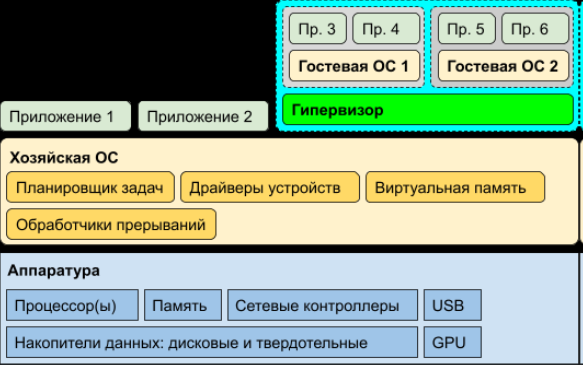
\includegraphics[width=1\textwidth]{1.png}}\\ 
    \small\textit{Рис.1 - Вывод top}  
    \label{framework} 
\end{figure}

Утилита отобразит текущее состояние процессов в колонке S(tate).
\begin{itemize}
    \item[-] \textbf{(R)} Процесс в настоящее время активен и использует процессорное время или находится в
    очереди работоспособных процессов, ожидающих получения услуг.
    \item[-] \textbf{(S)} Процесс ожидает завершения события.
    \item[-] \textbf{(D)} Процесс находится в спящем состоянии, и его нельзя остановить. Обычно это происходит,
    когда процесс ожидает ввода-вывода.
    \item[-] \textbf{(T)} Процесс был остановлен, что обычно происходит с интерактивным процессом оболочки, с
    помощью последовательности клавиш Ctrl-Z.
    \item[-] \textbf{(Z)} Процесс был остановлен, но не может быть удален его родительским элементом, который
    перешел в неуправляемое состояние.
\end{itemize}

Важный параметр, который можно увидеть справа сверху, - это load average, который выражается как
количество процессов, находящихся в рабочем состоянии (R) или в состоянии блокировки (D).
Средняя нагрузка отображается за последние 1, 5 и 15 минут. 
\ \textbf{Важно!} \ \underbar{\textit{Как \ показывает}} \\
\underbar{\textit{практика, средняя загрузка не должна превышать количество ядер CPU}} \\
\underbar{\textit{в системе. Вы можете узнать количество ядер с помощью команды}} \\
\underbar{\textit{\textbf{lscpu}.}}\\

С помощью top легко увидеть процессы, на которые стоит обратить внимание. Исходя из рисунка 1,
можно сделать вывод, что созданная ранее служба сильно нагружает систему, так как потребляет
почти 100\% CPU. С помощью нажатия на \textbf{k} можно передать сигнал прямо из top.\\

Выбираем номер процесса и номер сигнала для передачи.
\vspace{0.3cm}

\begin{lstlisting}
PID to signal/kill [default pid = 20462]
    PID USER     PR NI    VIRT   RES   SHR S %CPU %MEM      TIME+ COMMAND
  20462 root     20  0    5520   780   720 R 93.8   0.0  55:00.66 dd

Send pid 20462 signal [15/sigterm]
    PID USER     PR NI    VIRT   RES   SHR S %CPU %MEM      TIME+ COMMAND
  20462 root     20  0    5520   780   720 R 93.8   0.0  55:00.66 dd
$$
\end{lstlisting}
\vspace{0.3cm}

Состояние процесса следует оценивать не только по загрузке системы, но и по сообщениям, которые
запущенные службы записывают. Процессы могут быть в нормальном с точки зрения потребления
ресурсов состоянии, но в логах окажутся ошибки о невозможности выполнения заложенных действий.
Ранее мы рассмотрели файлы логов, расположенные в каталоге \textbf{/var/log}, но помимо этого существует
сервис \textbf{systemd-journald}, который хранит сообщения в журнале, двоичном файле \textbf{/run/log/journal}.
Этот файл можно просмотреть с помощью команды \textbf{journalctl}.\\

Самый простой способ использовать \textbf{journalctl} - просто ввести команду.

\vspace{0.3cm}
\begin{lstlisting}
root@server:$\sim$# journalctl
-- Logs begin at Mon 2020-12-07 17:59:17 UTC, end at Sun 2021-01-10 
15:25:29 UTC. --
Dec   07   17:59:17   server   kernel:   Linux  version  5.4.0-56-generic
(buildd@lgw01-amd64-025) (gcc version 9.3.0 (Ubuntu 9.3.0-17ubuntu1$\sim$20.04
))
#62-Ubuntu SMP Mon Nov 23 19:20:19 UTC 2020 (Ubuntu 5.4.0-56.62-g>
Dec    07   17:59:17   server   kernel:   Command
      line: BOOT_IMAGE=/vmlinuz-5.4.0-56-generic root=/dev/mapper/ubuntu--
vg-ubuntu--lv ro Dec 07 17:59:17 server kernel: KERNEL supported cpus:
Dec 07 17:59:17 server          Intel GenuineIntel
kernel:                         AMD AuthenticAMD
Dec 07 17:59:17 server          Hygon HygonGenuine
kernel:                         Centaur CentaurHauls
Dec 07 17:59:17 server          zhaoxi    Shangha
kernel:
$$
\end{lstlisting}
\vspace{0.2cm}

Поскольку журнал ведется с момента загрузки сервера, в начале отображаются сообщения,
связанные с загрузкой. Если вы хотите увидеть последние сообщения, которые были
зарегистрированы, вы можете использовать G (в верхнем регистре), чтобы перейти в конец журнала,
или опцию \textbf{-f} для просмотра наполнения журнала в реальном времени.\\

Одна из полезных функций - это возможность отсортировать ошибки.

\vspace{0.3cm}
\begin{lstlisting}
root@server:$\sim$# journalctl -p err
-- Logs begin at Mon 2020-12-07 17:59:17 UTC, end at Sun 2021-01-10 
15:25:29 UTC. --
Dec 07 17:59:17 server   kernel: [drm:vmw_host_log [vmwgfx]] *ERROR* 
Failed to send host log message.   
Dec 07 17:59:17 server   kernel: [drm:vmw_host_log [vmwgfx]] *ERROR*
Failed to send host log message.  
Dec 08 07:52:51 server   systemd-networkd-wait-online[3163]: Event loop 
failed: Connection timed out
Dec 08 07:54:04 server   systemd-networkd-wait-online[3609]: Event loop
failed: Connection timed out

...
\end{lstlisting}
\vspace{0.2cm}

Или сообщения, относящиеся к определенной службе.

\vspace{0.3cm}
\begin{lstlisting}
root@server:$\sim$# journalctl -u nginx
-- Logs begin at Mon 2020-12-07 17:59:17 UTC, end at Sun 2021-01-10 
15:25:29 UTC. --
Dec 17 17:24:17 server systemd[1]: Starting A high performance web server 
and a reverse proxy server...
Dec 17 17:24:17 server systemd[1]: Started A high performance web server 
and a reverse proxy server.
Dec 17 17:24:31 server systemd[1]: Stopping A high performance web server 
and a reverse proxy server...
Dec 17 17:24:31 server systemd[1]: nginx.service: Succeeded.
Dec 17 17:24:31 server systemd[1]: Stopped A high performance web server 
and a reverse proxy server.
Dec 17 17:26:41 server systemd[1]: Starting A high performance web server 
and a reverse proxy server...
Dec 17 17:26:41 server systemd[1]: Started A high performance web server 
and a reverse proxy server.
\end{lstlisting}
\vspace{0.2cm}

\textbf{Важно!} \underbar{\textit{Журнал очищается при перезагрузке системы. Чтобы жур-}} \\
\underbar{\textit{нал оставался постоянным между перезагрузками, необходимо наличие}} \\
\underbar{\textit{каталога \textbf{/var/log/journal}, а так же параметр \textbf{Storage=auto} в \textbf{/etc/}}} \\ 
\underbar{\textit{\textbf{systemd/journal.conf}}}.

\newpage

\section*{Практическое задание} 
\addcontentsline{toc}{section}{Практическое задание}

\begin{enumerate}
    \item Изменить конфигурационный файл службы SSH: /etc/ssh/sshd\_config, отключив
    аутентификацию по паролю PasswordAuthentication no. Выполните рестарт службы \colorbox{backcolour}{systemctl
    restart sshd (service sshd restart)}, верните аутентификацию по паролю, выполните
    reload службы \colorbox{backcolour}{systemctl} \colorbox{backcolour}{reload sshd (service sshd reload)}. В чём различие между
    действиями restart и reload?
    \item Установить программу mc с помощью apt-get install -y mc. Запустите mc. Используя ps, найдите
    PID процесса, завершите процесс, передав ему сигнал 9.
    \item Создать юнит нового процесса с именем userping, который при старте будет выполнять ping
    адреса 127.0.0.1.\\
    Сделать так, чтобы команда запускалась сразу при старте операционной системы.
    Запустить сервис с помощью systemctl, отследить pid процесса, остановить процесс с
    помощью сигналов в top.
\end{enumerate}

\section*{Глоссарий} 
\addcontentsline{toc}{section}{Глоссарий}

\href{https://ru.wikipedia.org/wiki/Загрузчик_операционной_системы}{\underbar{\textbf{Загрузчик}}} — программное обеспечение, обеспечивающее загрузку операционной системы сразу
после включения компьютера или сервера.\\

\noindent \href{https://ru.wikipedia.org/wiki/Ядро_Linux}{\underbar{\textbf{Ядро}}} — центральная часть операционной системы, обеспечивающая приложениям доступ к
ресурсам компьютера (ресурсам центрального процессора, памяти и т. д.).\\

\noindent \href{https://ru.wikipedia.org/wiki/Initrd}{\underbar{\textbf{Initrd}}} — виртуальная файловая система, используемая ядром ОС Linux перед монтированием
файловых систем. На этой файловой системе могут находиться модули или какие-то особые
параметры служб, которые необходимы для корректного старта ОС.\\

\noindent \href{https://ru.wikipedia.org/wiki/Systemd}{\underbar{\textbf{Systemd}}} — система инициализации Linux, процесс для запуска юнитов (элементарных единиц в
терминологии systemd) в Linux и управления ими в процессе работы системы. Его особенность —
интенсивное распараллеливание запуска служб в процессе загрузки системы, что позволяет
существенно ускорить запуск операционной системы.\\

\noindent \href{https://ru.wikipedia.org/wiki/Процесс_(информатика)}{\underbar{\textbf{Процесс}}} — набор программного кода, выполняемого в памяти компьютера.\\

\noindent \href{https://ru.wikipedia.org/wiki/Компьютерная_программа}{\underbar{\textbf{Приложение}}} — программное обеспечение, включающее в себя исполняемый код, конфигурационные
файлы, данные.\\

\noindent \href{https://wm-help.net/lib/b/book/1696396857/275}{\underbar{\textbf{Таблица процессов}}} — структура данных, описывающая все процессы, запущенные в данный момент
в операционной системе, их PID, состояние, строку команды.

\section*{Дополнительные материалы} 
\addcontentsline{toc}{section}{Дополнительные материалы}

\href{https://habr.com/ru/post/423049/}{\textit{Процессы в Linux}}

\section*{Используемые источники} 
\addcontentsline{toc}{section}{Используемые источники}

\href{https://habr.com/ru/post/113350/}{\textit{Загрузка операционной системы}}\\

\noindent \href{https://www.linuxcenter.ru/lib/articles/system/linux_processes.phtml}{\textit{Процессы в Linux}}\\

\noindent \href{https://it.wikireading.ru/6468}{\textit{Робачевский А. Операционная система Unix}}\\

\noindent \href{https://www.linuxcenter.ru/lib/books/kostromin}{\textit{Костромин В. Linux для пользователя}}



\end{document}